\documentclass[12pt,]{article}
\usepackage{lmodern}
\usepackage{amssymb,amsmath}
\usepackage{ifxetex,ifluatex}
\usepackage{fixltx2e} % provides \textsubscript
\ifnum 0\ifxetex 1\fi\ifluatex 1\fi=0 % if pdftex
  \usepackage[T1]{fontenc}
  \usepackage[utf8]{inputenc}
\else % if luatex or xelatex
  \ifxetex
    \usepackage{mathspec}
  \else
    \usepackage{fontspec}
  \fi
  \defaultfontfeatures{Ligatures=TeX,Scale=MatchLowercase}
    \setmainfont[]{Times New Roman}
\fi
% use upquote if available, for straight quotes in verbatim environments
\IfFileExists{upquote.sty}{\usepackage{upquote}}{}
% use microtype if available
\IfFileExists{microtype.sty}{%
\usepackage{microtype}
\UseMicrotypeSet[protrusion]{basicmath} % disable protrusion for tt fonts
}{}
\usepackage[margin=2.54cm]{geometry}
\usepackage{hyperref}
\hypersetup{unicode=true,
            pdftitle={Study of Temporal and Spatial Generation Patterns of U.S. Power Plants},
            pdfauthor={Xin Zhang},
            pdfborder={0 0 0},
            breaklinks=true}
\urlstyle{same}  % don't use monospace font for urls
\usepackage{color}
\usepackage{fancyvrb}
\newcommand{\VerbBar}{|}
\newcommand{\VERB}{\Verb[commandchars=\\\{\}]}
\DefineVerbatimEnvironment{Highlighting}{Verbatim}{commandchars=\\\{\}}
% Add ',fontsize=\small' for more characters per line
\usepackage{framed}
\definecolor{shadecolor}{RGB}{248,248,248}
\newenvironment{Shaded}{\begin{snugshade}}{\end{snugshade}}
\newcommand{\KeywordTok}[1]{\textcolor[rgb]{0.13,0.29,0.53}{\textbf{#1}}}
\newcommand{\DataTypeTok}[1]{\textcolor[rgb]{0.13,0.29,0.53}{#1}}
\newcommand{\DecValTok}[1]{\textcolor[rgb]{0.00,0.00,0.81}{#1}}
\newcommand{\BaseNTok}[1]{\textcolor[rgb]{0.00,0.00,0.81}{#1}}
\newcommand{\FloatTok}[1]{\textcolor[rgb]{0.00,0.00,0.81}{#1}}
\newcommand{\ConstantTok}[1]{\textcolor[rgb]{0.00,0.00,0.00}{#1}}
\newcommand{\CharTok}[1]{\textcolor[rgb]{0.31,0.60,0.02}{#1}}
\newcommand{\SpecialCharTok}[1]{\textcolor[rgb]{0.00,0.00,0.00}{#1}}
\newcommand{\StringTok}[1]{\textcolor[rgb]{0.31,0.60,0.02}{#1}}
\newcommand{\VerbatimStringTok}[1]{\textcolor[rgb]{0.31,0.60,0.02}{#1}}
\newcommand{\SpecialStringTok}[1]{\textcolor[rgb]{0.31,0.60,0.02}{#1}}
\newcommand{\ImportTok}[1]{#1}
\newcommand{\CommentTok}[1]{\textcolor[rgb]{0.56,0.35,0.01}{\textit{#1}}}
\newcommand{\DocumentationTok}[1]{\textcolor[rgb]{0.56,0.35,0.01}{\textbf{\textit{#1}}}}
\newcommand{\AnnotationTok}[1]{\textcolor[rgb]{0.56,0.35,0.01}{\textbf{\textit{#1}}}}
\newcommand{\CommentVarTok}[1]{\textcolor[rgb]{0.56,0.35,0.01}{\textbf{\textit{#1}}}}
\newcommand{\OtherTok}[1]{\textcolor[rgb]{0.56,0.35,0.01}{#1}}
\newcommand{\FunctionTok}[1]{\textcolor[rgb]{0.00,0.00,0.00}{#1}}
\newcommand{\VariableTok}[1]{\textcolor[rgb]{0.00,0.00,0.00}{#1}}
\newcommand{\ControlFlowTok}[1]{\textcolor[rgb]{0.13,0.29,0.53}{\textbf{#1}}}
\newcommand{\OperatorTok}[1]{\textcolor[rgb]{0.81,0.36,0.00}{\textbf{#1}}}
\newcommand{\BuiltInTok}[1]{#1}
\newcommand{\ExtensionTok}[1]{#1}
\newcommand{\PreprocessorTok}[1]{\textcolor[rgb]{0.56,0.35,0.01}{\textit{#1}}}
\newcommand{\AttributeTok}[1]{\textcolor[rgb]{0.77,0.63,0.00}{#1}}
\newcommand{\RegionMarkerTok}[1]{#1}
\newcommand{\InformationTok}[1]{\textcolor[rgb]{0.56,0.35,0.01}{\textbf{\textit{#1}}}}
\newcommand{\WarningTok}[1]{\textcolor[rgb]{0.56,0.35,0.01}{\textbf{\textit{#1}}}}
\newcommand{\AlertTok}[1]{\textcolor[rgb]{0.94,0.16,0.16}{#1}}
\newcommand{\ErrorTok}[1]{\textcolor[rgb]{0.64,0.00,0.00}{\textbf{#1}}}
\newcommand{\NormalTok}[1]{#1}
\usepackage{longtable,booktabs}
\usepackage{graphicx,grffile}
\makeatletter
\def\maxwidth{\ifdim\Gin@nat@width>\linewidth\linewidth\else\Gin@nat@width\fi}
\def\maxheight{\ifdim\Gin@nat@height>\textheight\textheight\else\Gin@nat@height\fi}
\makeatother
% Scale images if necessary, so that they will not overflow the page
% margins by default, and it is still possible to overwrite the defaults
% using explicit options in \includegraphics[width, height, ...]{}
\setkeys{Gin}{width=\maxwidth,height=\maxheight,keepaspectratio}
\IfFileExists{parskip.sty}{%
\usepackage{parskip}
}{% else
\setlength{\parindent}{0pt}
\setlength{\parskip}{6pt plus 2pt minus 1pt}
}
\setlength{\emergencystretch}{3em}  % prevent overfull lines
\providecommand{\tightlist}{%
  \setlength{\itemsep}{0pt}\setlength{\parskip}{0pt}}
\setcounter{secnumdepth}{5}
% Redefines (sub)paragraphs to behave more like sections
\ifx\paragraph\undefined\else
\let\oldparagraph\paragraph
\renewcommand{\paragraph}[1]{\oldparagraph{#1}\mbox{}}
\fi
\ifx\subparagraph\undefined\else
\let\oldsubparagraph\subparagraph
\renewcommand{\subparagraph}[1]{\oldsubparagraph{#1}\mbox{}}
\fi

%%% Use protect on footnotes to avoid problems with footnotes in titles
\let\rmarkdownfootnote\footnote%
\def\footnote{\protect\rmarkdownfootnote}

%%% Change title format to be more compact
\usepackage{titling}

% Create subtitle command for use in maketitle
\providecommand{\subtitle}[1]{
  \posttitle{
    \begin{center}\large#1\end{center}
    }
}

\setlength{\droptitle}{-2em}

  \title{Study of Temporal and Spatial Generation Patterns of U.S. Power Plants}
    \pretitle{\vspace{\droptitle}\centering\huge}
  \posttitle{\par}
  \subtitle{\url{https://github.com/zhangxsaras/eGRID16}}
  \author{Xin Zhang}
    \preauthor{\centering\large\emph}
  \postauthor{\par}
    \date{}
    \predate{}\postdate{}
  

\begin{document}
\maketitle
\begin{abstract}
Power plant emissions contribute a great amount Green House Gas (GHG) to
the atmosphere and GHG emissions account a lot for the global mean
temperature rise. Power Plant emission amount is related to its
generation and in general, higher generation indicates higher fuel use
and higher emission. Studying power plants generation can help us
understand emission pattern. To study the temporal and spatial pattern
of power plants generation can help us predict future power generation
and then we can give suggestions accordingly to reduce emission. I used
the Emissions \& Generation Resource Integrated Database (eGRID) to do
analysis. From the time series analysis and spatial analysis results, it
turned out there is an installation time trend for generator annual net
generation, and there are spatial distribution patterns of power plants
in U.S.. From 1900s to 2016, the generation increased with fluctuation
and the trend was related to policy and world fuel market. We could not
predict the future electricity generation since there was no clear trend
after 1987. However, from the differences of spatial distribution
patterns of Power Plants in U.S., we found that using renewable energy
to replace traditional energy power plants can help a lot to reduce GHG
emission in the future.
\end{abstract}

\newpage

\tableofcontents  \newpage
\listoftables  \newpage
\listoffigures  \newpage

\textless{}Note: set up autoreferencing for figures and tables in your
document\textgreater{}

\section{Research Question and
Rationale}\label{research-question-and-rationale}

\begin{quote}
Public awareness of global climate change's impacts on the environment
and the society has increased. Greenhouse gas (GHG) emissions account a
lot for the global mean temperature rise. To achieve the goal of
limiting global warming to 1.5°C, by 2030, global net human-caused
emissions of carbon dioxide (CO2) would need to decrease by around 45 \%
from 2010 levels, and by 2050, CO2 emission would need to reach `net
zero' (IPCC, 2018). In United States, a large amount of GHG emissions
come from the electric power sector. The electric power sector accounts
for 38\% of the total U.S. energy consumption in 2017 (US EIA, 2017). In
the same year, the transportation end-use sector and other mobile
combustion accounted for 1,732.02 MMT CO2Eq., which accounts 28\% of the
total GHG emission in the U.S., which is the second largest GHG
emissions from all other sectors (the largest is the transportation
sector) (US EPA, 2018). To study the temporal and spatial pattern of
power plants generation can help us predict future power generation and
then we can give suggestions accordingly to reduce emission.
\end{quote}

\begin{quote}
Therefore, here I raise two research questions: (1) Is there an
installation time trend for generator annual net generation? (New power
generators tend to have higher or lower capacity overtime?) (2) Is there
a spatial distribution pattern of Power Plants in U.S.? (Number of power
plants/ Total Electricity Generation/ Equivalent CO2 emission in each
state \textasciitilde{} States)
\end{quote}

\begin{quote}
Here I am going to use the 2016 Emissions \& Generation Resource
Integrated Database (eGRID). It is a comprehensive source of data on the
environmental characteristics of \# almost all electric power generated
in the United States. I am going to use the GEN16 tab (2016 Generators)
and the PLNT 16 tab (2016 Plants). (Note: usually one power plant has
several generators). The former gives information of all the generators
currently in use in 2016 and the latter gives information of all the
power plants in use in 2016.
\end{quote}

\newpage

\section{Dataset Information}\label{dataset-information}

\begin{quote}
Here I am going to use the 2016 Emissions \& Generation Resource
Integrated Database (eGRID). It is a comprehensive source of data on the
environmental characteristics of \# almost all electric power generated
in the United States. I am going to use the GEN16 tab (2016 Generators)
and the PLNT 16 tab (2016 Plants). The dataset was retrieved at:
\url{https://www.epa.gov/energy/emissions-generation-resource-integrated-database-egrid}
on 2019-03-25 21:10:11 EDT. It was originally an excel file and I saved
it as two separate csv files of GEN16 an PLNT16. Since the dataset has
two names in the first two rows (one full name and one abbreviate one),
here I only list the columns I will use later, others can check the
original dataset for references.
\end{quote}

\begin{quote}
\begin{longtable}[]{@{}llllll@{}}
\caption{Dataset Information}\tabularnewline
\toprule
\begin{minipage}[b]{0.14\columnwidth}\raggedright\strut
Dataset Name\strut
\end{minipage} & \begin{minipage}[b]{0.14\columnwidth}\raggedright\strut
Information\strut
\end{minipage} & \begin{minipage}[b]{0.14\columnwidth}\raggedright\strut
Useful Column1\strut
\end{minipage} & \begin{minipage}[b]{0.14\columnwidth}\raggedright\strut
Useful Column2\strut
\end{minipage} & \begin{minipage}[b]{0.14\columnwidth}\raggedright\strut
Useful Column3\strut
\end{minipage} & \begin{minipage}[b]{0.14\columnwidth}\raggedright\strut
Useful Column4\strut
\end{minipage}\tabularnewline
\midrule
\endfirsthead
\toprule
\begin{minipage}[b]{0.14\columnwidth}\raggedright\strut
Dataset Name\strut
\end{minipage} & \begin{minipage}[b]{0.14\columnwidth}\raggedright\strut
Information\strut
\end{minipage} & \begin{minipage}[b]{0.14\columnwidth}\raggedright\strut
Useful Column1\strut
\end{minipage} & \begin{minipage}[b]{0.14\columnwidth}\raggedright\strut
Useful Column2\strut
\end{minipage} & \begin{minipage}[b]{0.14\columnwidth}\raggedright\strut
Useful Column3\strut
\end{minipage} & \begin{minipage}[b]{0.14\columnwidth}\raggedright\strut
Useful Column4\strut
\end{minipage}\tabularnewline
\midrule
\endhead
\begin{minipage}[t]{0.14\columnwidth}\raggedright\strut
GEN16\strut
\end{minipage} & \begin{minipage}[t]{0.14\columnwidth}\raggedright\strut
Generators Information\strut
\end{minipage} & \begin{minipage}[t]{0.14\columnwidth}\raggedright\strut
SEQGEN16: eGRID2016 Plant file sequence number\strut
\end{minipage} & \begin{minipage}[t]{0.14\columnwidth}\raggedright\strut
PSTATABB: Plant state abbreviation\strut
\end{minipage} & \begin{minipage}[t]{0.14\columnwidth}\raggedright\strut
GENNTAN: Generator annual net generation (MWh)\strut
\end{minipage} & \begin{minipage}[t]{0.14\columnwidth}\raggedright\strut
GENYRONL: Generator year on-line\strut
\end{minipage}\tabularnewline
\begin{minipage}[t]{0.14\columnwidth}\raggedright\strut
PLNT16\strut
\end{minipage} & \begin{minipage}[t]{0.14\columnwidth}\raggedright\strut
Plants Information\strut
\end{minipage} & \begin{minipage}[t]{0.14\columnwidth}\raggedright\strut
SEQGEN16: eGRID2016 Plant file sequence number\strut
\end{minipage} & \begin{minipage}[t]{0.14\columnwidth}\raggedright\strut
PSTATABB: Plant state abbreviation\strut
\end{minipage} & \begin{minipage}[t]{0.14\columnwidth}\raggedright\strut
PLNGENAN: Plant annual net generation (MWh)\strut
\end{minipage} & \begin{minipage}[t]{0.14\columnwidth}\raggedright\strut
PLCO2EQA: Plant annual CO2 equivalent emissions (tons)\strut
\end{minipage}\tabularnewline
\bottomrule
\end{longtable}
\end{quote}

\newpage

\section{Exploratory Data Analysis and
Wrangling}\label{exploratory-data-analysis-and-wrangling}

\begin{Shaded}
\begin{Highlighting}[]
\CommentTok{#Load dataset}
\NormalTok{GEN16 <-}\StringTok{ }\KeywordTok{read.csv}\NormalTok{(}\StringTok{"./Data/Raw/egrid_GEN16.csv"}\NormalTok{)}
\NormalTok{PLNT16 <-}\StringTok{ }\KeywordTok{read.csv}\NormalTok{(}\StringTok{"./Data/Raw/egrid_PLNT16.csv"}\NormalTok{)}

\CommentTok{#data wrangling}
\CommentTok{#This dataset has two names, one is the full name, and the first row is the abbreviation}
\CommentTok{#change column names to the abbr.}
\KeywordTok{names}\NormalTok{(GEN16) <-}\StringTok{ }\KeywordTok{lapply}\NormalTok{(GEN16[}\DecValTok{1}\NormalTok{, ], as.character)}
\KeywordTok{names}\NormalTok{(PLNT16) <-}\StringTok{ }\KeywordTok{lapply}\NormalTok{(PLNT16[}\DecValTok{1}\NormalTok{, ], as.character)}

\CommentTok{#filter out the first row and use abbr. as column names}
\NormalTok{GEN16 <-}\StringTok{ }\NormalTok{GEN16[}\DecValTok{2}\OperatorTok{:}\DecValTok{26184}\NormalTok{,] }
\NormalTok{PLNT16 <-}\StringTok{ }\NormalTok{PLNT16[}\DecValTok{2}\OperatorTok{:}\DecValTok{9710}\NormalTok{,]}


\CommentTok{#numeric data has comma, convert factor to numberic}
\KeywordTok{class}\NormalTok{ (GEN16}\OperatorTok{$}\NormalTok{GENNTAN)}
\end{Highlighting}
\end{Shaded}

\begin{verbatim}
## [1] "factor"
\end{verbatim}

\begin{Shaded}
\begin{Highlighting}[]
\NormalTok{GEN16}\OperatorTok{$}\NormalTok{GENNTAN <-}\KeywordTok{as.numeric}\NormalTok{(}\KeywordTok{gsub}\NormalTok{(}\StringTok{","}\NormalTok{, }\StringTok{""}\NormalTok{, GEN16}\OperatorTok{$}\NormalTok{GENNTAN))}
\NormalTok{PLNT16}\OperatorTok{$}\NormalTok{PLNGENAN <-}\KeywordTok{as.numeric}\NormalTok{(}\KeywordTok{gsub}\NormalTok{(}\StringTok{","}\NormalTok{, }\StringTok{""}\NormalTok{, PLNT16}\OperatorTok{$}\NormalTok{PLNGENAN))}
\NormalTok{PLNT16}\OperatorTok{$}\NormalTok{PLCO2EQA <-}\KeywordTok{as.numeric}\NormalTok{(}\KeywordTok{gsub}\NormalTok{(}\StringTok{","}\NormalTok{, }\StringTok{""}\NormalTok{, PLNT16}\OperatorTok{$}\NormalTok{PLCO2EQA))}

\CommentTok{#Year data as.Date}
\KeywordTok{class}\NormalTok{ (GEN16}\OperatorTok{$}\NormalTok{GENYRONL)}
\end{Highlighting}
\end{Shaded}

\begin{verbatim}
## [1] "factor"
\end{verbatim}

\begin{Shaded}
\begin{Highlighting}[]
\NormalTok{GEN16}\OperatorTok{$}\NormalTok{GENYRONL<-}\KeywordTok{as.Date}\NormalTok{(GEN16}\OperatorTok{$}\NormalTok{GENYRONL,}\DataTypeTok{format =} \StringTok{"%Y"}\NormalTok{)}

\CommentTok{#filter data by the sequence of time}
\NormalTok{GEN16 =}\StringTok{ }\NormalTok{GEN16[}\KeywordTok{order}\NormalTok{(GEN16[,}\StringTok{'GENYRONL'}\NormalTok{]),]}

\CommentTok{#GEN16 - sum the totoal generation by year}
\NormalTok{GEN16sel <-}\StringTok{ }\NormalTok{GEN16 }\OperatorTok
\StringTok{  }\KeywordTok{select}\NormalTok{(SEQGEN16, PSTATABB, GENNTAN, GENYRONL) }\OperatorTok
\StringTok{  }\KeywordTok{filter}\NormalTok{(}\OperatorTok{!}\KeywordTok{is.na}\NormalTok{(GENNTAN)) }\OperatorTok
\StringTok{  }\KeywordTok{filter}\NormalTok{(GENNTAN}\OperatorTok{>}\DecValTok{0}\NormalTok{) }\OperatorTok
\StringTok{  }\KeywordTok{group_by}\NormalTok{(GENYRONL)}\OperatorTok
\StringTok{  }\KeywordTok{summarise}\NormalTok{(}\DataTypeTok{GENSUM =} \KeywordTok{sum}\NormalTok{(GENNTAN)) }

\CommentTok{#PLNT16 - sum the totoal generation/CO2/plant numbers by state}
\NormalTok{PLNT16sel <-}\StringTok{ }\NormalTok{PLNT16 }\OperatorTok
\StringTok{  }\KeywordTok{select}\NormalTok{(SEQPLT16, PSTATABB, PLPRMFL, PLNGENAN, PLCO2EQA) }\OperatorTok
\StringTok{    }\KeywordTok{filter}\NormalTok{(}\OperatorTok{!}\KeywordTok{is.na}\NormalTok{(PLNGENAN)}\OperatorTok{&!}\KeywordTok{is.na}\NormalTok{(PLCO2EQA)) }\OperatorTok
\StringTok{  }\KeywordTok{filter}\NormalTok{(PLNGENAN}\OperatorTok{>}\DecValTok{0}\NormalTok{)}\OperatorTok
\StringTok{  }\KeywordTok{group_by}\NormalTok{(PSTATABB)}\OperatorTok
\StringTok{  }\KeywordTok{summarise}\NormalTok{(}\DataTypeTok{PLNTGEN =} \KeywordTok{sum}\NormalTok{(PLNGENAN),}
            \DataTypeTok{ECO2 =} \KeywordTok{sum}\NormalTok{(PLCO2EQA),}
            \DataTypeTok{Count=}\KeywordTok{n}\NormalTok{())}

\CommentTok{#summary code for GEN16}
\KeywordTok{colnames}\NormalTok{(GEN16sel)}
\end{Highlighting}
\end{Shaded}

\begin{verbatim}
## [1] "GENYRONL" "GENSUM"
\end{verbatim}

\begin{Shaded}
\begin{Highlighting}[]
\KeywordTok{class}\NormalTok{(GEN16sel}\OperatorTok{$}\NormalTok{GENSUM)}
\end{Highlighting}
\end{Shaded}

\begin{verbatim}
## [1] "numeric"
\end{verbatim}

\begin{Shaded}
\begin{Highlighting}[]
\KeywordTok{class}\NormalTok{(GEN16sel}\OperatorTok{$}\NormalTok{GENNTAN)}
\end{Highlighting}
\end{Shaded}

\begin{verbatim}
## Warning: Unknown or uninitialised column: 'GENNTAN'.
\end{verbatim}

\begin{verbatim}
## [1] "NULL"
\end{verbatim}

\begin{Shaded}
\begin{Highlighting}[]
\KeywordTok{summary}\NormalTok{(GEN16sel)}
\end{Highlighting}
\end{Shaded}

\begin{verbatim}
##     GENYRONL              GENSUM         
##  Min.   :1891-04-15   Min.   :      876  
##  1st Qu.:1925-10-14   1st Qu.:   794214  
##  Median :1956-04-15   Median : 10767508  
##  Mean   :1956-03-21   Mean   : 33200403  
##  3rd Qu.:1986-10-14   3rd Qu.: 60662462  
##  Max.   :2017-04-15   Max.   :213550203
\end{verbatim}

\begin{Shaded}
\begin{Highlighting}[]
\KeywordTok{dim}\NormalTok{(GEN16sel)}
\end{Highlighting}
\end{Shaded}

\begin{verbatim}
## [1] 123   2
\end{verbatim}

\begin{Shaded}
\begin{Highlighting}[]
\KeywordTok{head}\NormalTok{(GEN16sel)}
\end{Highlighting}
\end{Shaded}

\begin{verbatim}
## # A tibble: 6 x 2
##   GENYRONL   GENSUM
##   <date>      <dbl>
## 1 1891-04-15  24330
## 2 1893-04-15   1512
## 3 1896-04-15  21453
## 4 1898-04-15  25514
## 5 1899-04-15    876
## 6 1900-04-15  20899
\end{verbatim}

\begin{Shaded}
\begin{Highlighting}[]
\CommentTok{#summary code for PLNT16}
\KeywordTok{colnames}\NormalTok{(PLNT16sel)}
\end{Highlighting}
\end{Shaded}

\begin{verbatim}
## [1] "PSTATABB" "PLNTGEN"  "ECO2"     "Count"
\end{verbatim}

\begin{Shaded}
\begin{Highlighting}[]
\KeywordTok{class}\NormalTok{(PLNT16sel}\OperatorTok{$}\NormalTok{PLNTGEN)}
\end{Highlighting}
\end{Shaded}

\begin{verbatim}
## [1] "numeric"
\end{verbatim}

\begin{Shaded}
\begin{Highlighting}[]
\KeywordTok{class}\NormalTok{(PLNT16sel}\OperatorTok{$}\NormalTok{ECO2)}
\end{Highlighting}
\end{Shaded}

\begin{verbatim}
## [1] "numeric"
\end{verbatim}

\begin{Shaded}
\begin{Highlighting}[]
\KeywordTok{summary}\NormalTok{(PLNT16sel)}
\end{Highlighting}
\end{Shaded}

\begin{verbatim}
##     PSTATABB     PLNTGEN               ECO2               Count       
##  AK     : 1   Min.   :    76474   Min.   :    18470   Min.   :   2.0  
##  AL     : 1   1st Qu.: 34625868   1st Qu.: 11970062   1st Qu.:  61.0  
##  AR     : 1   Median : 60445059   Median : 31234830   Median :  96.0  
##  AZ     : 1   Mean   : 80006416   Mean   : 40119484   Mean   : 146.5  
##  CA     : 1   3rd Qu.:107747773   3rd Qu.: 54001623   3rd Qu.: 148.0  
##  CO     : 1   Max.   :453941341   Max.   :239363582   Max.   :1163.0  
##  (Other):45
\end{verbatim}

\begin{Shaded}
\begin{Highlighting}[]
\KeywordTok{dim}\NormalTok{(PLNT16sel)}
\end{Highlighting}
\end{Shaded}

\begin{verbatim}
## [1] 51  4
\end{verbatim}

\begin{Shaded}
\begin{Highlighting}[]
\KeywordTok{head}\NormalTok{(PLNT16sel)}
\end{Highlighting}
\end{Shaded}

\begin{verbatim}
## # A tibble: 6 x 4
##   PSTATABB   PLNTGEN     ECO2 Count
##   <fct>        <dbl>    <dbl> <int>
## 1 AK         6339538  2944890   128
## 2 AL       142863565 65536193    69
## 3 AR        60445059 33927595    52
## 4 AZ       108734651 50946063   112
## 5 CA       197956373 44797489  1163
## 6 CO        54679959 40213412   147
\end{verbatim}

\begin{Shaded}
\begin{Highlighting}[]
\CommentTok{#save new datasets}
\CommentTok{#write.csv(GEN16sel, file = "./Data/Processed/GEN16sel_Processed.csv",row.names=FALSE)}
\CommentTok{#write.csv(PLNT16sel, file = "./Data/Processed/PLNT16sel_Processed.csv",row.names=FALSE)}
\CommentTok{#data prep for shiny app}
\CommentTok{#PLNT16orisel <- PLNT16 %>%}
\CommentTok{#  select(SEQPLT16, PSTATABB, PLPRMFL, PLNGENAN, PLCO2EQA) %>%}
\CommentTok{#    filter(!is.na(PLNGENAN)&!is.na(PLCO2EQA)) %>%}
\CommentTok{#  filter(PLNGENAN>0)}
\CommentTok{#write.csv(PLNT16orisel, file = "./Data/Processed/PLNT16ori_Processed.csv",row.names=FALSE)}
\end{Highlighting}
\end{Shaded}

\begin{figure}
\centering
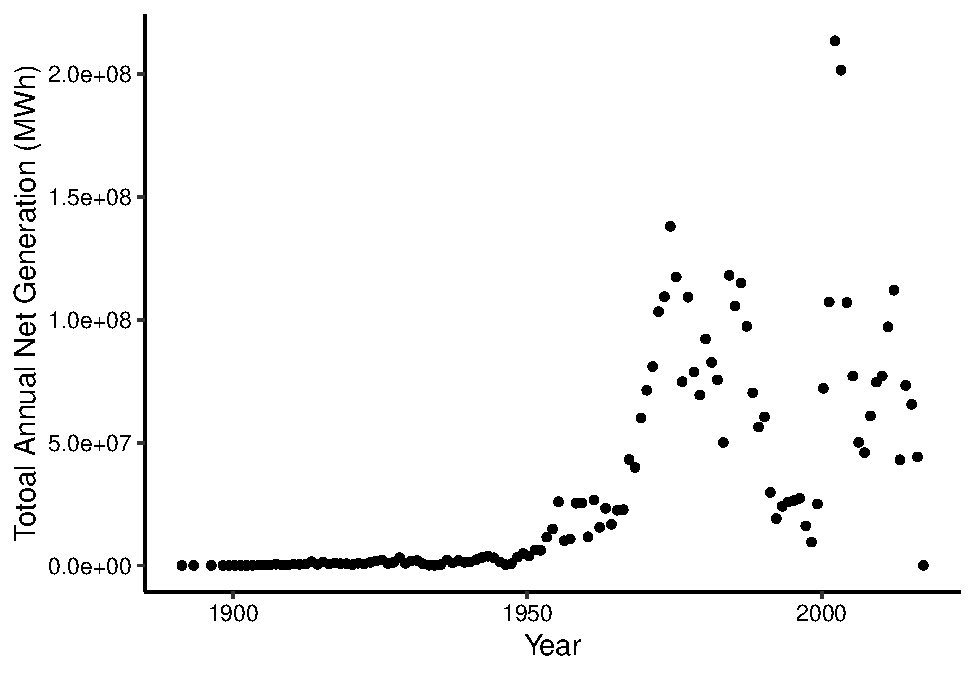
\includegraphics{Zhang_X_ENV872_Project_files/figure-latex/unnamed-chunk-2-1.pdf}
\caption{Overview of Generator online year}
\end{figure}

\begin{figure}
\centering
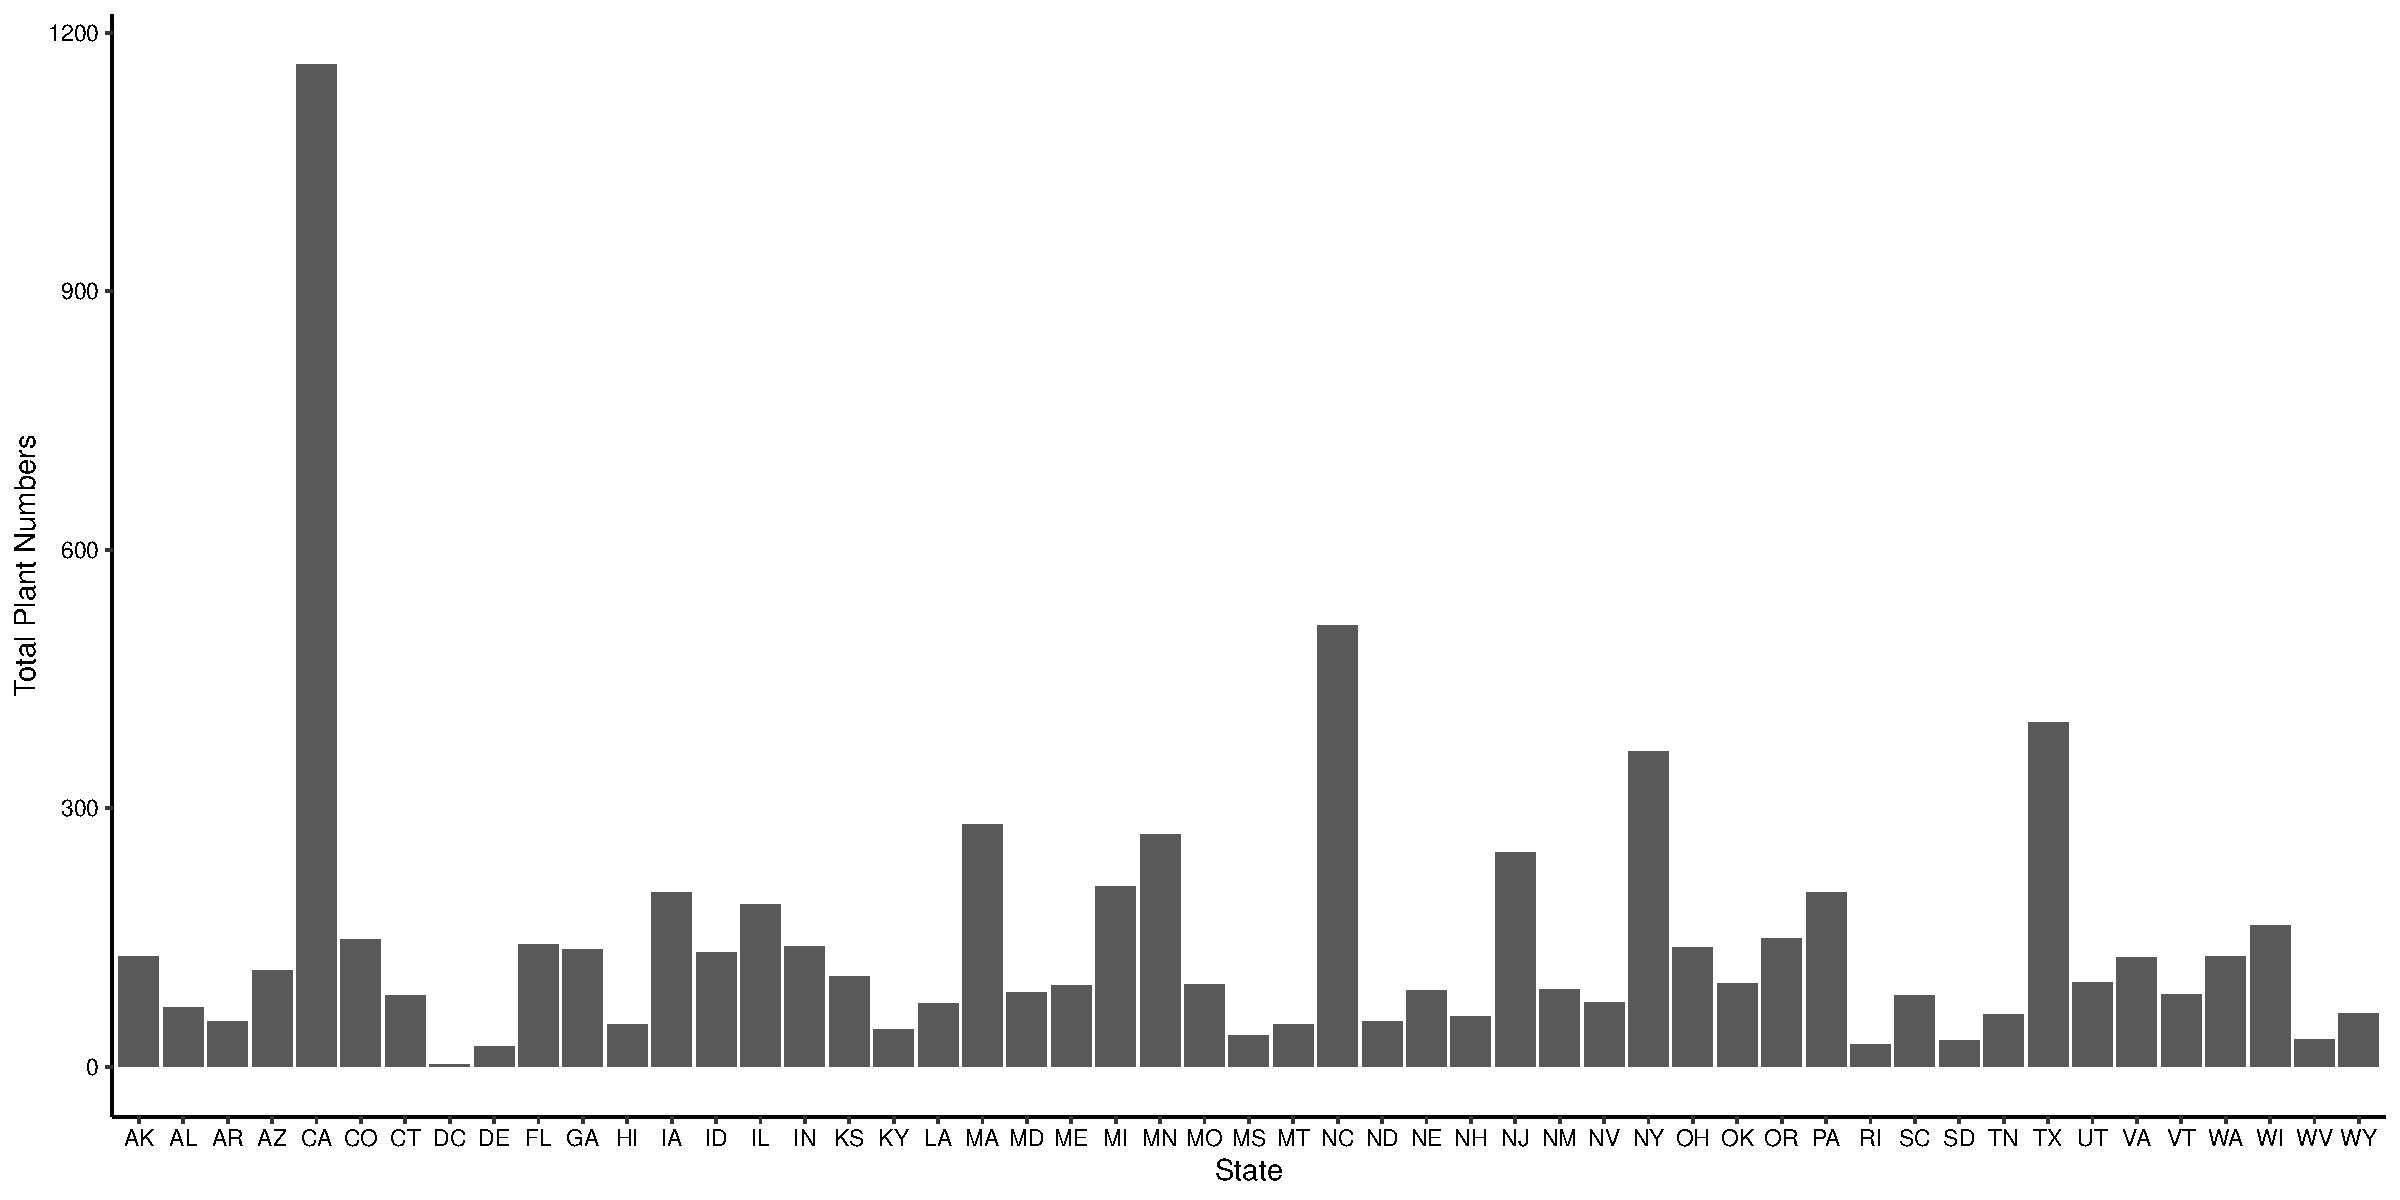
\includegraphics{Zhang_X_ENV872_Project_files/figure-latex/unnamed-chunk-3-1.pdf}
\caption{Plant Numbers}
\end{figure}

\begin{figure}
\centering
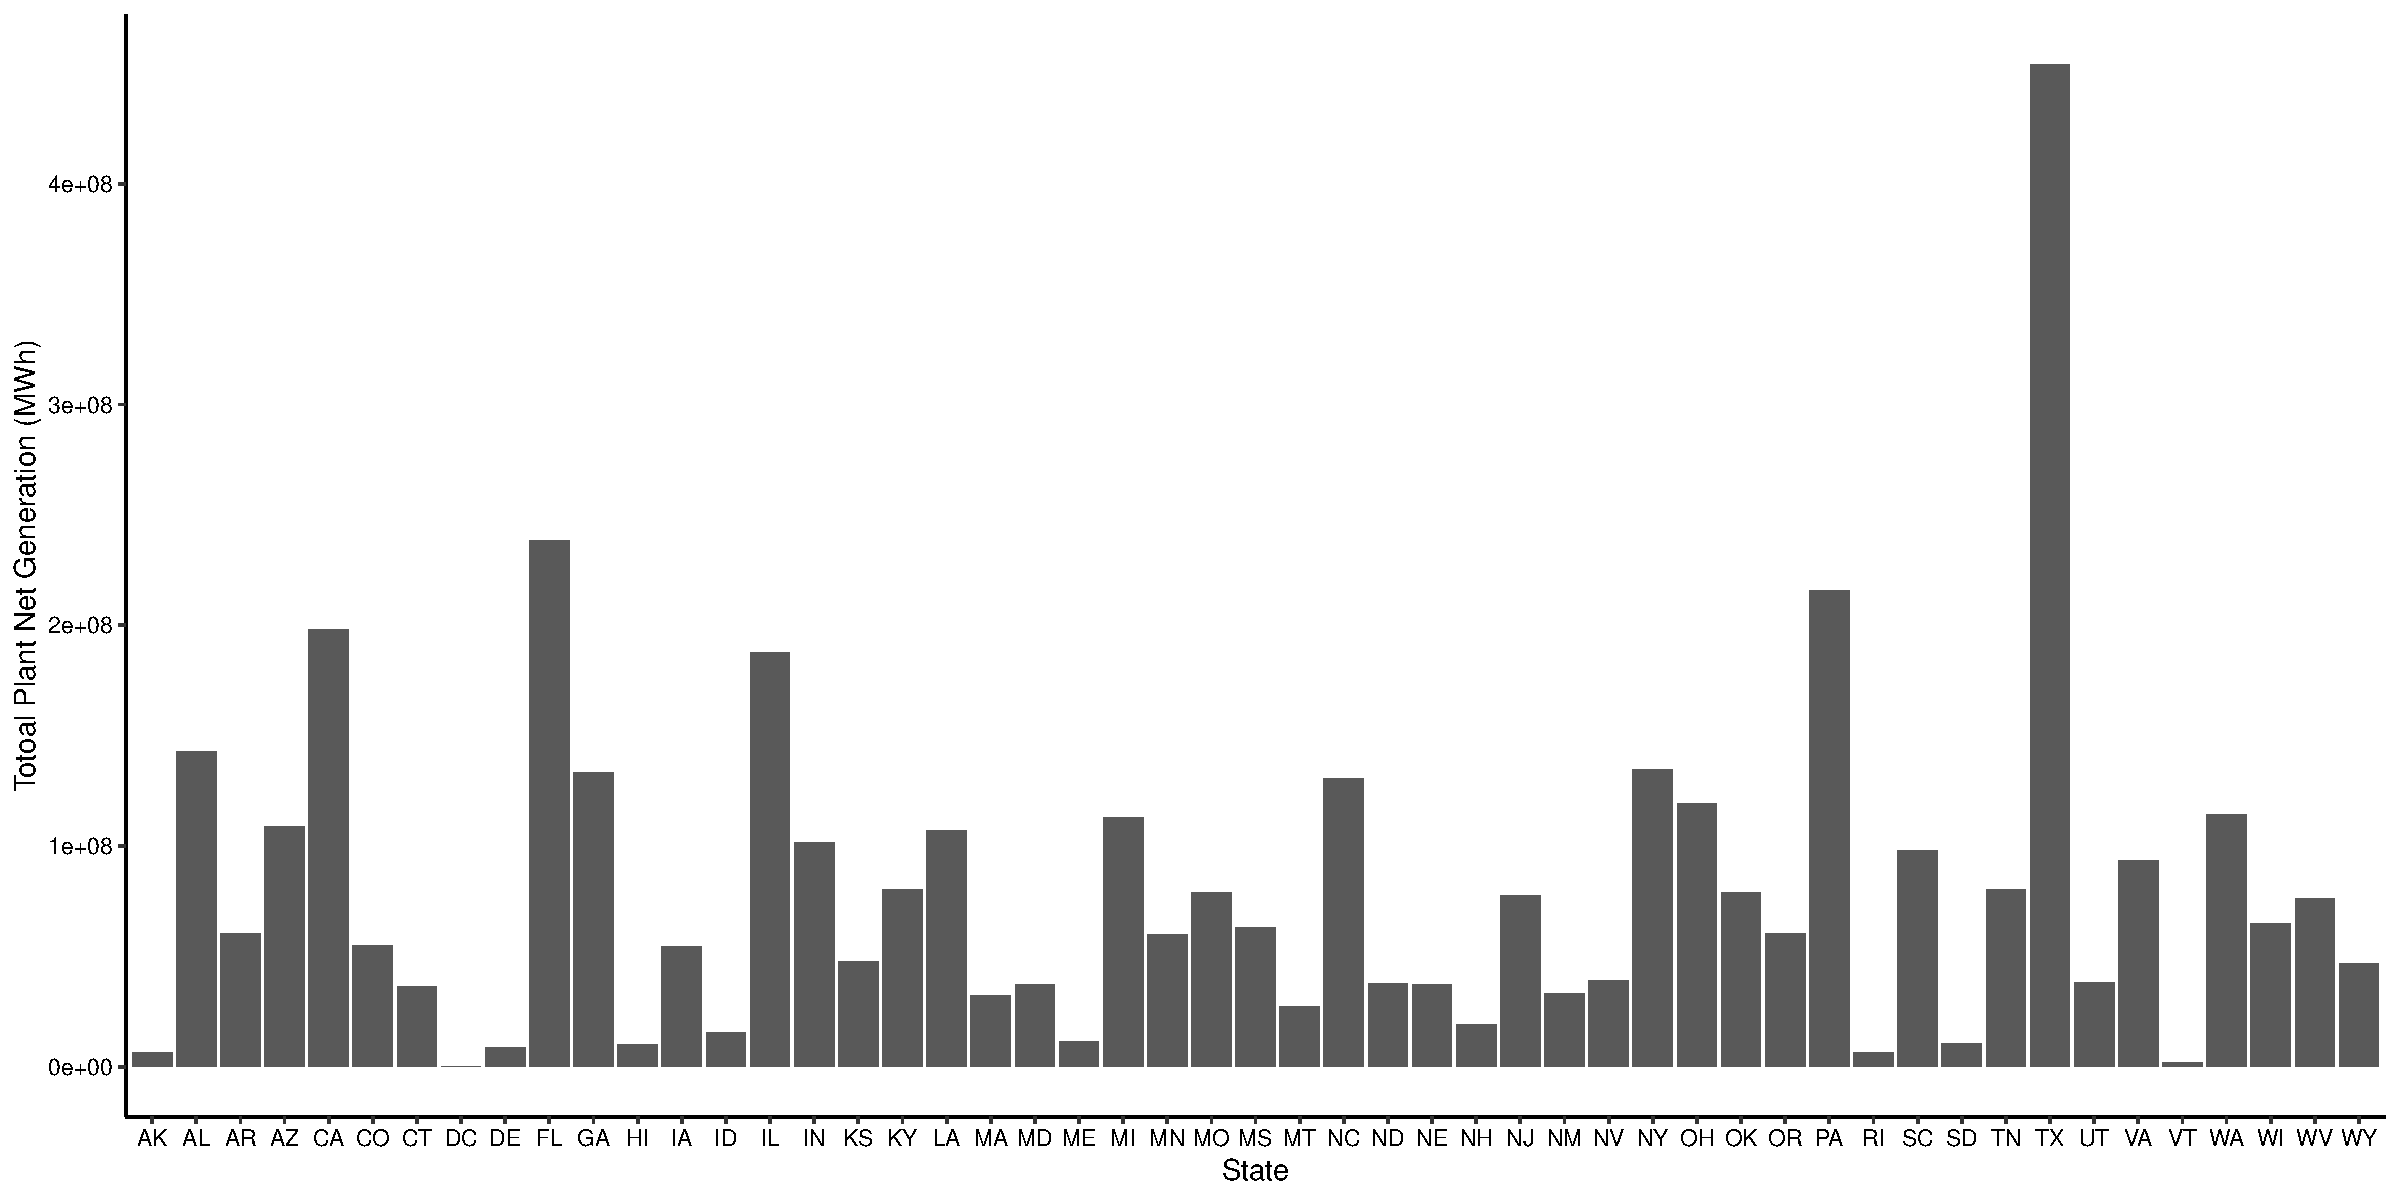
\includegraphics{Zhang_X_ENV872_Project_files/figure-latex/unnamed-chunk-4-1.pdf}
\caption{Plant Generation}
\end{figure}

\begin{figure}
\centering
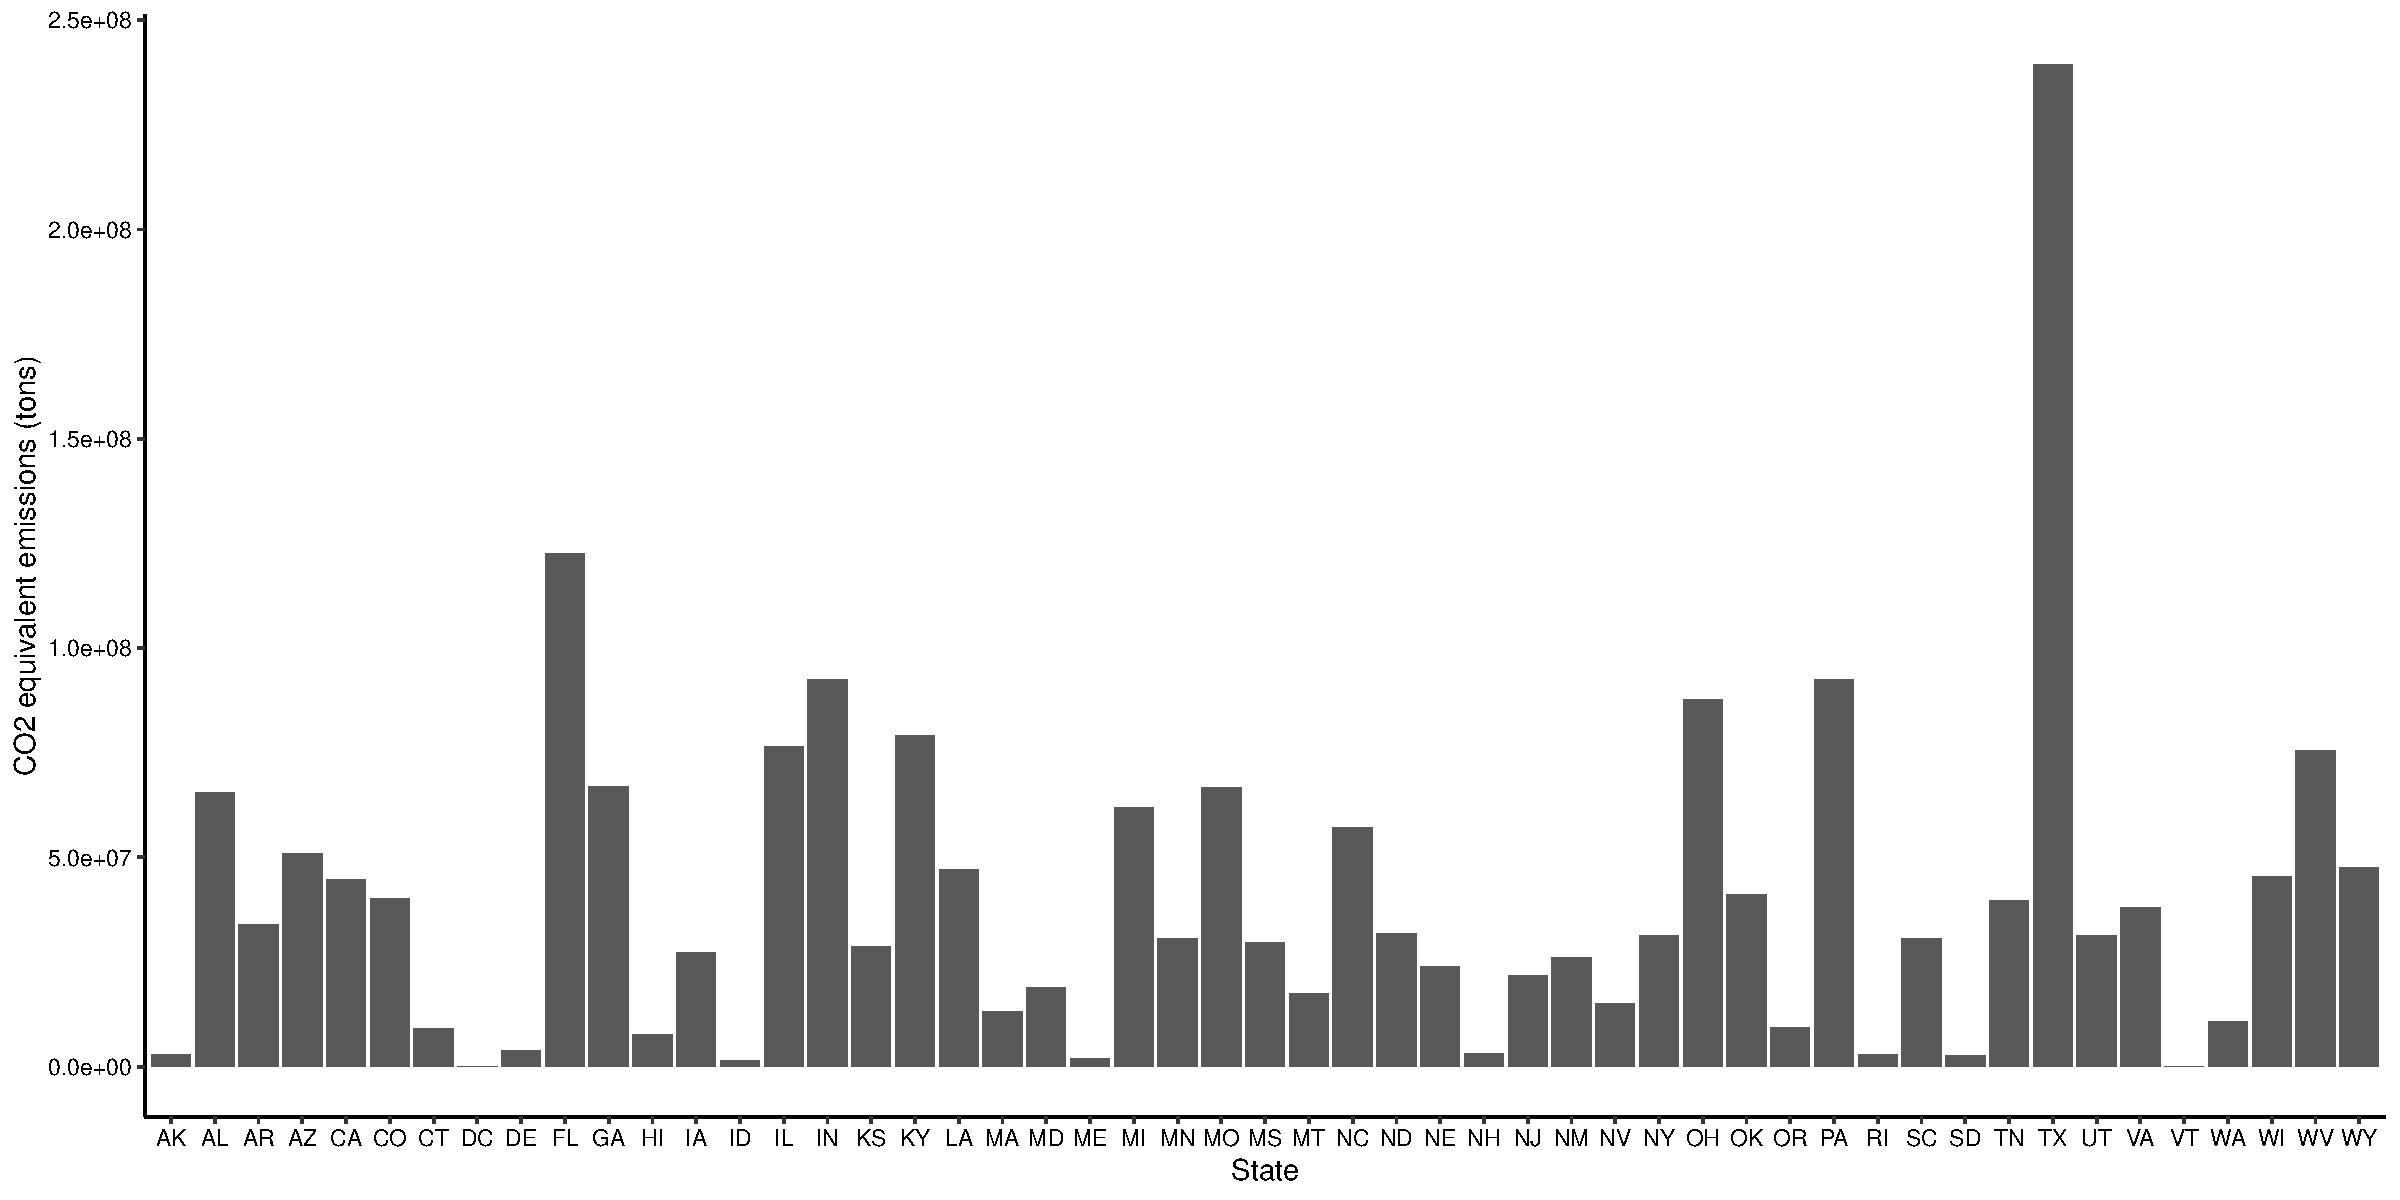
\includegraphics{Zhang_X_ENV872_Project_files/figure-latex/unnamed-chunk-5-1.pdf}
\caption{Plant Equivalent CO2 Emissions}
\end{figure}

\newpage

\section{Analysis}\label{analysis}

\begin{Shaded}
\begin{Highlighting}[]
\CommentTok{#Q1 Time series analysis on GEN16}
\CommentTok{# Use GLM to see if there is a significant time trend}
\NormalTok{GENTest.fixed <-}\StringTok{ }\KeywordTok{gls}\NormalTok{(}\DataTypeTok{data =}\NormalTok{ GEN16sel,}
\NormalTok{                     GENSUM }\OperatorTok{~}\StringTok{ }\NormalTok{GENYRONL, }
                      \DataTypeTok{method =} \StringTok{"REML"}\NormalTok{)}
\KeywordTok{summary}\NormalTok{(GENTest.fixed) }\CommentTok{# significnat trend t=10.23, p<0.005.}
\end{Highlighting}
\end{Shaded}

\begin{verbatim}
## Generalized least squares fit by REML
##   Model: GENSUM ~ GENYRONL 
##   Data: GEN16sel 
##        AIC      BIC    logLik
##   4562.782 4571.169 -2278.391
## 
## Coefficients:
##                Value Std.Error  t-value p-value
## (Intercept) 44750764 3129296.8 14.30058       0
## GENYRONL        2295     224.3 10.22992       0
## 
##  Correlation: 
##          (Intr)
## GENYRONL 0.361 
## 
## Standardized residuals:
##        Min         Q1        Med         Q3        Max 
## -2.6061370 -0.5704619 -0.1403653  0.3843417  4.3789847 
## 
## Residual standard error: 32367813 
## Degrees of freedom: 123 total; 121 residual
\end{verbatim}

\begin{quote}
According to GLM, time has a significant effect on the total annual net
generation of generators (t=10.23, p\textless{}0.05).
\end{quote}

\begin{Shaded}
\begin{Highlighting}[]
\CommentTok{# Run a Mann-Kendall test}
\KeywordTok{mk.test}\NormalTok{(GEN16sel}\OperatorTok{$}\NormalTok{GENSUM)}
\end{Highlighting}
\end{Shaded}

\begin{verbatim}
## 
##  Mann-Kendall trend test
## 
## data:  GEN16sel$GENSUM
## z = 11.311, n = 123, p-value < 2.2e-16
## alternative hypothesis: true S is not equal to 0
## sample estimates:
##            S         varS          tau 
## 5.175000e+03 2.092503e+05 6.897241e-01
\end{verbatim}

\begin{Shaded}
\begin{Highlighting}[]
\CommentTok{# there is a trend over time according to this test (p<0.001), Z is positive, positive trend - time passes, value increases }

\CommentTok{# Test for change point}
\KeywordTok{pettitt.test}\NormalTok{(GEN16sel}\OperatorTok{$}\NormalTok{GENSUM) }\CommentTok{#changing point at 58 - Year 1952}
\end{Highlighting}
\end{Shaded}

\begin{verbatim}
## 
##  Pettitt's test for single change-point detection
## 
## data:  GEN16sel$GENSUM
## U* = 3670, p-value < 2.2e-16
## alternative hypothesis: two.sided
## sample estimates:
## probable change point at time K 
##                              58
\end{verbatim}

\begin{Shaded}
\begin{Highlighting}[]
\CommentTok{#GEN16sel[58,]}

\CommentTok{# Run separate Mann-Kendall for each change point}
\KeywordTok{mk.test}\NormalTok{(GEN16sel}\OperatorTok{$}\NormalTok{GENSUM[}\DecValTok{1}\OperatorTok{:}\DecValTok{57}\NormalTok{])}
\end{Highlighting}
\end{Shaded}

\begin{verbatim}
## 
##  Mann-Kendall trend test
## 
## data:  GEN16sel$GENSUM[1:57]
## z = 6.8907, n = 57, p-value = 5.551e-12
## alternative hypothesis: true S is not equal to 0
## sample estimates:
##            S         varS          tau 
## 1.002000e+03 2.110267e+04 6.278195e-01
\end{verbatim}

\begin{Shaded}
\begin{Highlighting}[]
\CommentTok{# there is a trend over time according to this test (p<0.001), Z is positive, positive trend - time passes, value increasess }
\KeywordTok{mk.test}\NormalTok{(GEN16sel}\OperatorTok{$}\NormalTok{GENSUM[}\DecValTok{58}\OperatorTok{:}\DecValTok{123}\NormalTok{])}
\end{Highlighting}
\end{Shaded}

\begin{verbatim}
## 
##  Mann-Kendall trend test
## 
## data:  GEN16sel$GENSUM[58:123]
## z = 2.8224, n = 66, p-value = 0.004767
## alternative hypothesis: true S is not equal to 0
## sample estimates:
##            S         varS          tau 
## 5.110000e+02 3.265167e+04 2.382284e-01
\end{verbatim}

\begin{Shaded}
\begin{Highlighting}[]
\CommentTok{# there is a trend over time according to this test (p<0.05), Z is positive, positive trend - time passes, value increasess }

\CommentTok{# Is there a second change point?}
\KeywordTok{pettitt.test}\NormalTok{(GEN16sel}\OperatorTok{$}\NormalTok{GENSUM[}\DecValTok{58}\OperatorTok{:}\DecValTok{123}\NormalTok{]) }\CommentTok{#there is! 17 - Year 1969}
\end{Highlighting}
\end{Shaded}

\begin{verbatim}
## 
##  Pettitt's test for single change-point detection
## 
## data:  GEN16sel$GENSUM[58:123]
## U* = 681, p-value = 0.0001447
## alternative hypothesis: two.sided
## sample estimates:
## probable change point at time K 
##                              17
\end{verbatim}

\begin{Shaded}
\begin{Highlighting}[]
\CommentTok{#GEN16sel[75,]}

\CommentTok{# Run separate Mann-Kendall for each change point}
\KeywordTok{mk.test}\NormalTok{(GEN16sel}\OperatorTok{$}\NormalTok{GENSUM[}\DecValTok{58}\OperatorTok{:}\DecValTok{74}\NormalTok{])}
\end{Highlighting}
\end{Shaded}

\begin{verbatim}
## 
##  Mann-Kendall trend test
## 
## data:  GEN16sel$GENSUM[58:74]
## z = 2.5951, n = 17, p-value = 0.009455
## alternative hypothesis: true S is not equal to 0
## sample estimates:
##           S        varS         tau 
##  64.0000000 589.3333333   0.4705882
\end{verbatim}

\begin{Shaded}
\begin{Highlighting}[]
\CommentTok{# there is a trend over time according to this test (p<0.05), Z is positive, positive trend - time passes, value increasess }
\KeywordTok{mk.test}\NormalTok{(GEN16sel}\OperatorTok{$}\NormalTok{GENSUM[}\DecValTok{75}\OperatorTok{:}\DecValTok{123}\NormalTok{])}
\end{Highlighting}
\end{Shaded}

\begin{verbatim}
## 
##  Mann-Kendall trend test
## 
## data:  GEN16sel$GENSUM[75:123]
## z = -2.0084, n = 49, p-value = 0.0446
## alternative hypothesis: true S is not equal to 0
## sample estimates:
##             S          varS           tau 
##  -234.0000000 13458.6666667    -0.1989796
\end{verbatim}

\begin{Shaded}
\begin{Highlighting}[]
\CommentTok{# there is a trend over time according to this test (p<0.05), Z is negative, negative trend - time passes, value decreases }

\CommentTok{# Is there a third change point?}
\KeywordTok{pettitt.test}\NormalTok{(GEN16sel}\OperatorTok{$}\NormalTok{GENSUM[}\DecValTok{75}\OperatorTok{:}\DecValTok{123}\NormalTok{]) }\CommentTok{#there is! 1987}
\end{Highlighting}
\end{Shaded}

\begin{verbatim}
## 
##  Pettitt's test for single change-point detection
## 
## data:  GEN16sel$GENSUM[75:123]
## U* = 322, p-value = 0.01123
## alternative hypothesis: two.sided
## sample estimates:
## probable change point at time K 
##                              19
\end{verbatim}

\begin{Shaded}
\begin{Highlighting}[]
\CommentTok{# GEN16sel[94,]}
\KeywordTok{mk.test}\NormalTok{(GEN16sel}\OperatorTok{$}\NormalTok{GENSUM[}\DecValTok{75}\OperatorTok{:}\DecValTok{93}\NormalTok{]) }
\end{Highlighting}
\end{Shaded}

\begin{verbatim}
## 
##  Mann-Kendall trend test
## 
## data:  GEN16sel$GENSUM[75:93]
## z = 0.69971, n = 19, p-value = 0.4841
## alternative hypothesis: true S is not equal to 0
## sample estimates:
##          S       varS        tau 
##  21.000000 817.000000   0.122807
\end{verbatim}

\begin{Shaded}
\begin{Highlighting}[]
\CommentTok{# no trend!}
\KeywordTok{mk.test}\NormalTok{(GEN16sel}\OperatorTok{$}\NormalTok{GENSUM[}\DecValTok{94}\OperatorTok{:}\DecValTok{123}\NormalTok{])}
\end{Highlighting}
\end{Shaded}

\begin{verbatim}
## 
##  Mann-Kendall trend test
## 
## data:  GEN16sel$GENSUM[94:123]
## z = 1.1775, n = 30, p-value = 0.239
## alternative hypothesis: true S is not equal to 0
## sample estimates:
##           S        varS         tau 
##   67.000000 3141.666667    0.154023
\end{verbatim}

\begin{Shaded}
\begin{Highlighting}[]
\CommentTok{# no trend!}
\CommentTok{# no trend before and after the changing point}
\end{Highlighting}
\end{Shaded}

\begin{quote}
According to the Mann-Kendall test, there is a trend over time for total
annual net generation of generators (p\textless{}0.001), Z =11.311,
which indicates a positive trend over time. According to pettitt test.
There are three changing points: Year 1952, Year 1969 and Year 1987
(p\textless{}0.05).
\end{quote}

\begin{figure}
\centering
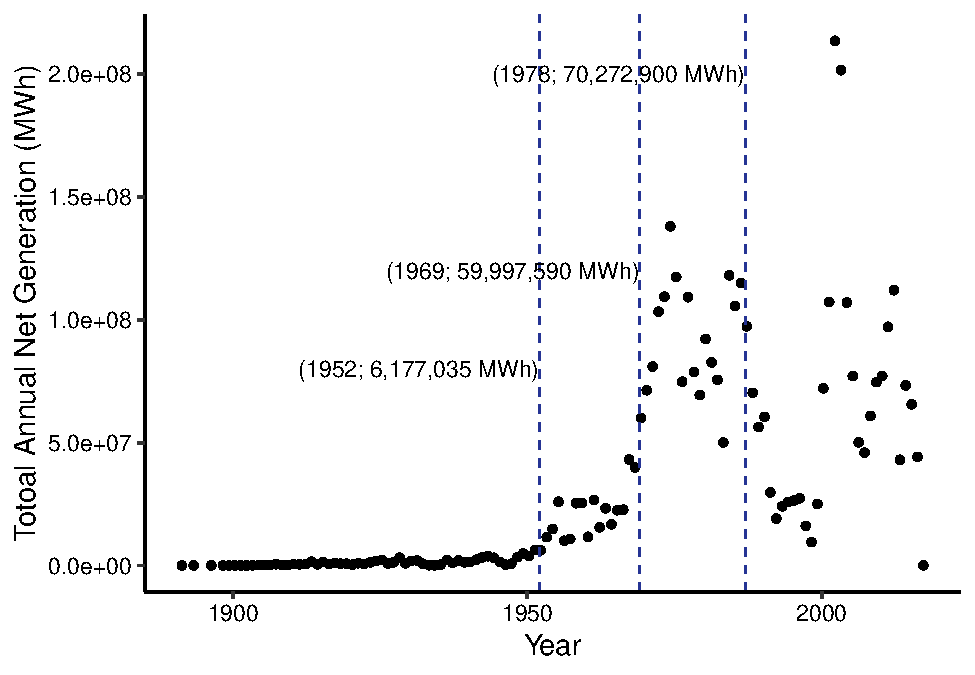
\includegraphics{Zhang_X_ENV872_Project_files/figure-latex/unnamed-chunk-8-1.pdf}
\caption{Generators Time Series Analysis}
\end{figure}

\begin{quote}
As is shown in the figure (Figure 5), before the first changing point
1952, the annual net generation of generators in U.S. increased very
slowly each year and after 1952, the speed of generation change became
faster. Annual net generation kept growing until 1969, this is the
second change point. After 1969, there was a negative trend of annual
net generation. The third changing point is Year 1987, and there was no
clear pattern in 1969-1987 or after 1987.
\end{quote}

\begin{Shaded}
\begin{Highlighting}[]
\CommentTok{#Q2 spatial distribution analysis on PLNT16}
\CommentTok{#data wrangling}
\CommentTok{#add fips number to PLNT16sel data}
\KeywordTok{library}\NormalTok{(usmap)}
\NormalTok{state_map <-}\StringTok{ }\KeywordTok{us_map}\NormalTok{(}\DataTypeTok{regions =} \StringTok{"states"}\NormalTok{)}
\NormalTok{PLNT_State<-}\StringTok{ }\KeywordTok{merge}\NormalTok{(state_map, PLNT16sel, }\DataTypeTok{by.x =} \StringTok{"abbr"}\NormalTok{, }\DataTypeTok{by.y =} \StringTok{"PSTATABB"}\NormalTok{)}\OperatorTok
\StringTok{   }\KeywordTok{select}\NormalTok{(abbr, fips, full, PLNTGEN, ECO2, Count)}
\NormalTok{PLNT_State =}\StringTok{ }\NormalTok{PLNT_State[}\OperatorTok{!}\KeywordTok{duplicated}\NormalTok{(PLNT_State}\OperatorTok{$}\NormalTok{abbr),]}

\CommentTok{#join PLNT16 data to counties map data}
\NormalTok{states_sf<-}\StringTok{ }\KeywordTok{st_read}\NormalTok{(}\StringTok{'./Data/RAW/States.shp'}\NormalTok{) }
\end{Highlighting}
\end{Shaded}

\begin{verbatim}
## Reading layer `States' from data source `C:\Users\Xin Zhang\Desktop\eGRID16\Data\Raw\States.shp' using driver `ESRI Shapefile'
## Simple feature collection with 52 features and 1 field
## geometry type:  MULTIPOLYGON
## dimension:      XY
## bbox:           xmin: -179.1743 ymin: 17.91377 xmax: 179.7739 ymax: 71.35256
## epsg (SRID):    4269
## proj4string:    +proj=longlat +datum=NAD83 +no_defs
\end{verbatim}

\begin{Shaded}
\begin{Highlighting}[]
\KeywordTok{st_crs}\NormalTok{(states_sf)}
\end{Highlighting}
\end{Shaded}

\begin{verbatim}
## Coordinate Reference System:
##   EPSG: 4269 
##   proj4string: "+proj=longlat +datum=NAD83 +no_defs"
\end{verbatim}

\begin{Shaded}
\begin{Highlighting}[]
\NormalTok{PLNT_State_merge <-}\StringTok{ }\KeywordTok{merge}\NormalTok{(states_sf, PLNT_State, }\DataTypeTok{by.x =} \StringTok{"STATEFP"}\NormalTok{, }\DataTypeTok{by.y =} \StringTok{"fips"}\NormalTok{)}
\CommentTok{#mapview(PLNT_State_merge)}
\end{Highlighting}
\end{Shaded}

\begin{figure}
\centering
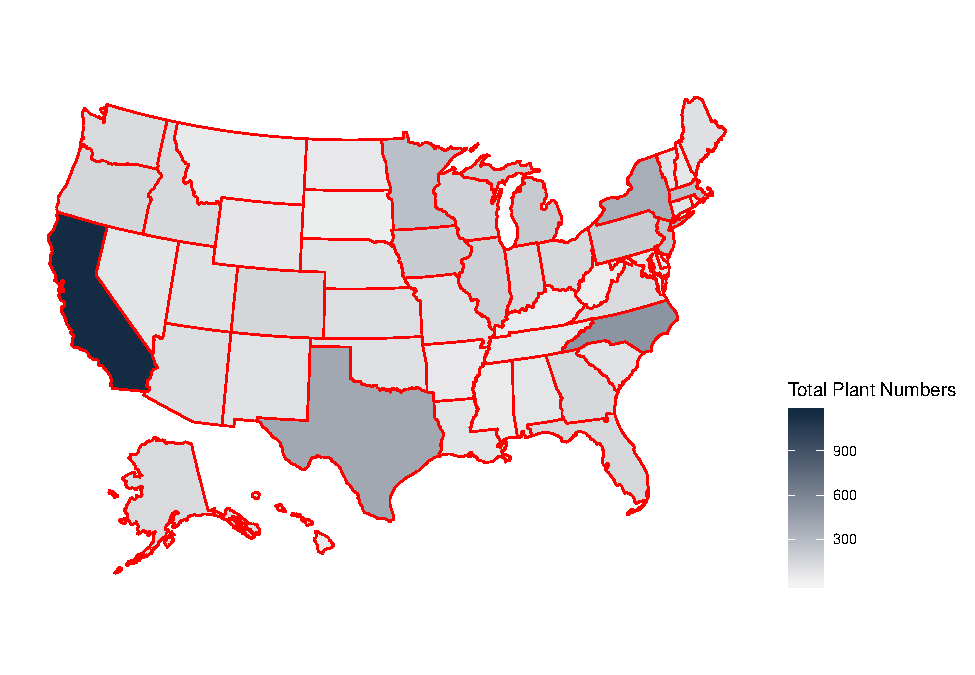
\includegraphics{Zhang_X_ENV872_Project_files/figure-latex/unnamed-chunk-10-1.pdf}
\caption{Map of Plant Numbers}
\end{figure}

\begin{figure}
\centering
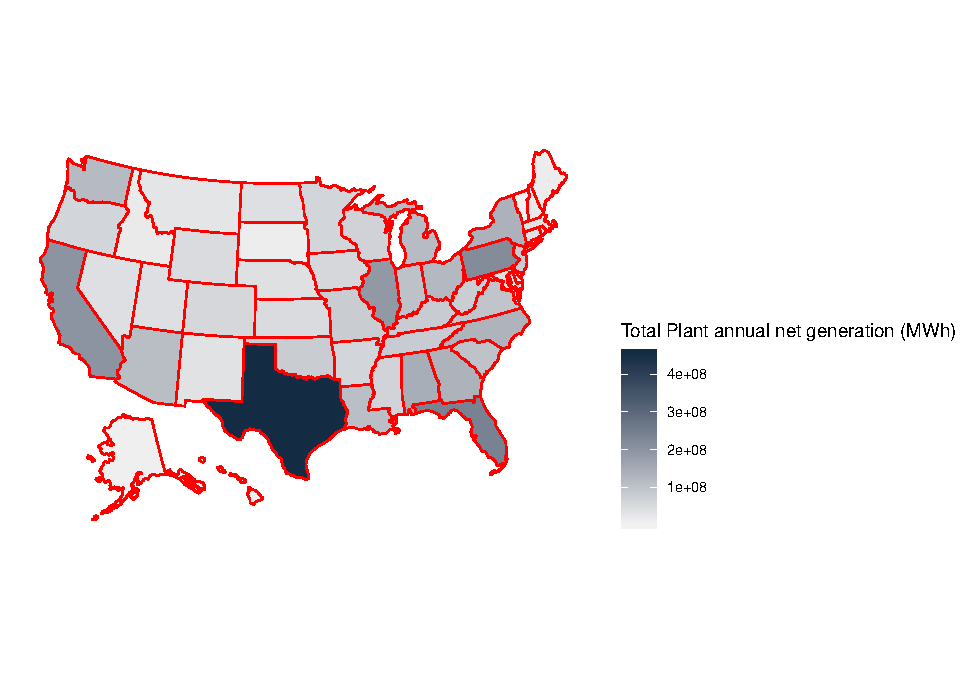
\includegraphics{Zhang_X_ENV872_Project_files/figure-latex/unnamed-chunk-11-1.pdf}
\caption{Map of Plant Generations}
\end{figure}

\begin{figure}
\centering
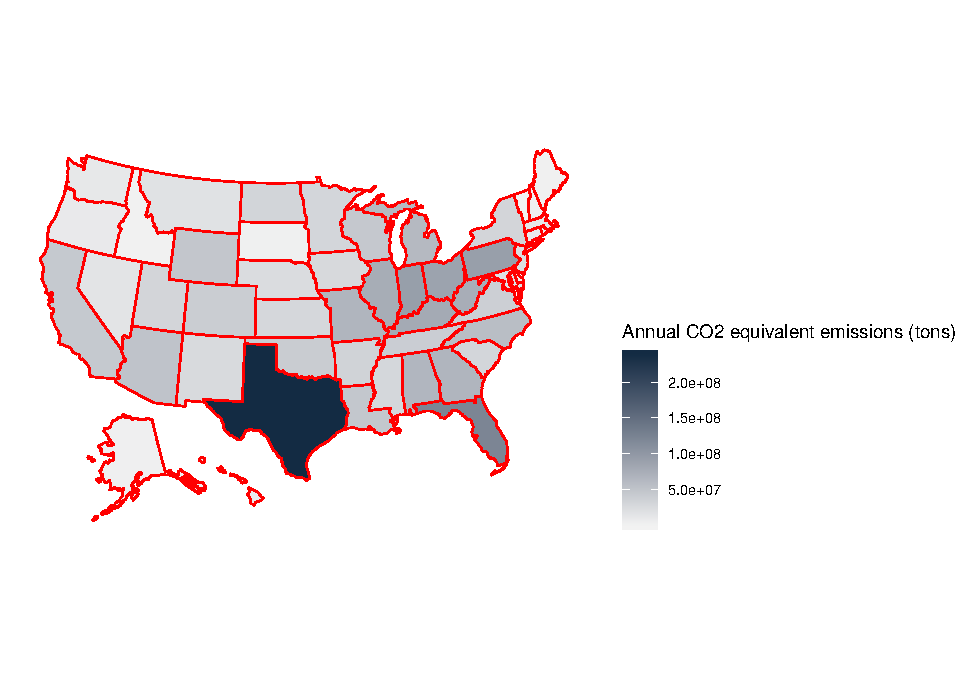
\includegraphics{Zhang_X_ENV872_Project_files/figure-latex/unnamed-chunk-12-1.pdf}
\caption{Map of Equivalent CO2 Emissions}
\end{figure}

\begin{quote}
Since our research scale is U.S., it also includes Alaska and this made
it very difficult to map it using ggplot (AL will be far away from other
states and the whole map will be very small to show). Therefore, here I
use the plot\_usmap function instead. As the maps show (Figure 6, 7, 8),
there are spatial distribution patterns. For total plant numbers,
California ranks first but in general, there are more power plants in
east coast states than in west coast. Texas is another exception in the
southern part that has relatively larger numbers of power plants. For
plant annual net generation, in general, east coast states also have
relatively higher net generation than west coast states, and Texas ranks
first. Accordingly, Texas also has highest annual CO2 equivalent
emissions, and east coast states have higher emissions than west coast
states.
\end{quote}

\newpage

\section{Summary and Conclusions}\label{summary-and-conclusions}

\begin{quote}
There are also three changing points of the whole period: 1952, 1969,
1987. After 1952, there is a huge increase in power generation each
year, this might be related to the technology thrive at the end of
1940s. The first hydraulic fracturing treatment was pumped on a gas well
operated by Pan American Petroleum Corp in the Hugoton field in 1947 and
it was the beginning of period of rapid electric industry growth
(Oilscams.org, Access: 2019-4-14). However, at the end of 1960s, energy
crisis caused the reduction of electricity generation and this energy
crisis peaked at 1973 (Energy Crisis (1970s), Access: 2019-4-14). This
accord with our second changing point here at 1969 and after 1969, there
was a negative trend of annual net generation.
\end{quote}

\begin{quote}
In the late 1970s, the government published more regulations on the
electricity generation industry such as the National Energy Act in 1978
to exert more control on the electricity industry. In 1990s, the
government published Congress passes Bush's Energy Policy Act (EPACT) to
deregulate the electricity industry (Ballotpedia, Access: 2019-4-14).
The back and force between strict and loose policies led to the
fluctuations of the generator generations, and this might be a cause why
there is a changing point of 1987 according to the pettitt test but
there was no trend before and after this year according to the
Mann-Kendall test.
\end{quote}

\begin{quote}
From the maps, we can see that there was spatial distribution pattern
for power plants generation in 2016. In general, eastern states had
higher power plant numbers, electricity net generation, and equivalent
CO2 emissions than western states. California ranked first for total
power plants numbers but its annual net generation and equivalent CO2
emission were both much less than Texas. The main reason for this was
the type of power plants. In Texas, there are more traditional power
plants using coal and natural gas as fuel, but in California, there are
more renewable energy power plants. Compared to traditional power plants
(600 MW, 0.75), renewable power plants have lower nameplate capacity and
capacity factor (1000MW, 0.1). Therefore, even though California had
more power plants, it had lower electricity generation. Also, compared
to traditional power plants, renewable power plants use clean energy and
barely have any emissions, so California's equivalent CO2 emissions were
also much lower than Texas.
\end{quote}

\begin{quote}
To sum up, there is an installation time trend for generator annual net
generation. From 1900s to 2016, the generation increased with
fluctuation and the trend was related to policy and world fuel market.
It was very difficult to predict the future electricity generation since
there was no clear trend after 1987. However, from the differences of
spatial distribution patterns of Power Plants in U.S., we can give
suggestions of using renewable energy to replace traditional energy
power plants. This can help a lot to reduce GHG emission in the future.
\end{quote}


\end{document}
